\documentclass{beamer}
\usepackage[T1]{fontenc}
\usepackage[brazil]{babel}
\usepackage[utf8]{inputenc}
\usepackage[document]{ragged2e}
\usetheme{Madrid}
\usecolortheme{default}
\definecolor{UBCblue}{rgb}{0.04706, 0.13725, 0.26667}
\definecolor{AccentGreen}{rgb}{0.11, 0.47, 0.30}
\definecolor{AccentRed}{rgb}{0.70, 0.15, 0.15}
\definecolor{LightGray}{rgb}{0.93, 0.93, 0.95}
\usepackage{graphicx}
% Os arquivos ficam nas pastas do artigo e dos diagramas; assim não duplicamos figuras.
\graphicspath{{.}{figs/}{../artigo/figuras/}{../artigo/figuras/zap/}{../diagramas/}}
\usepackage{listings}
\usepackage{subcaption}
\usecolortheme[named=UBCblue]{structure}
\usepackage{caption}
\usepackage{xcolor}
\usepackage{booktabs}
\usepackage{multirow}
\usepackage{array}
\usepackage{colortbl}
\usepackage{amsmath}
\usepackage{float}
\usepackage{tikz}
\usetikzlibrary{arrows.meta, positioning}

\setbeamertemplate{itemize items}[circle]
\setbeamertemplate{blocks}[rounded][shadow=true]
\setbeamertemplate{navigation symbols}{}

\makeatletter
\setbeamertemplate{footline}{%
  \leavevmode%
  \hbox{%
    \begin{beamercolorbox}[wd=.25\paperwidth,ht=2.25ex,dp=1ex,center]{author in head/foot}%
      \usebeamerfont{author in head/foot}\insertshortauthor
    \end{beamercolorbox}%
    \begin{beamercolorbox}[wd=.60\paperwidth,ht=2.25ex,dp=1ex,center]{title in head/foot}%
      \usebeamerfont{title in head/foot}\insertshortinstitute
    \end{beamercolorbox}%
  }%
  \begin{beamercolorbox}[wd=.15\paperwidth,ht=2.25ex,dp=1ex,right]{date in head/foot}%
    \usebeamerfont{date in head/foot}%
    \usebeamertemplate{page number in head/foot}%
    \hspace*{2ex}
  \end{beamercolorbox}
  \vskip0pt%
}
\makeatother

\author[Marlon B. Ramos]{Marlon Brendo Ramos}
\title[Engenharia de Software Seguro]{Engenharia de Software Seguro em um Sistema de
Faturamento de Redes Farmacêuticas, da
Modelagem de Ameaças ao DevSecOps}
\institute[UFU]{Universidade Federal de Uberlândia - UFU}
\date{}

\begin{document}
\frame{\titlepage}


\begin{frame}{Contexto e Motivação}
    \begin{itemize}
        \item \textbf{31\%} das violações começam pela exploração de vulnerabilidades de software.
(Fonte: \href{https://www.verizon.com/business/resources/reports/dbir/}{Verizon, 2026 DBIR}).
        \item No setor farmacêutico, os intermediários utilizam sistemas que registram informações, realizam cálculos e fazem as cobranças.
        \item \textbf{Change Healthcare (2024)}: acesso remoto \textbf{sem MFA} interrompeu pedidos e pagamentos em todo o território americano.
        \item Muitas falhas graves são de \textbf{projeto}, não de implementação. Um projeto inseguro não é corrigido por código perfeito.
    \end{itemize}

    \vspace{0.3cm}
    \begin{alertblock}{Ideia central}
        \centering
        Em vez de corrigir o que aparecer, perguntar \textbf{antes} como o sistema pode ser atacado.
    \end{alertblock}
\end{frame}

\begin{frame}{Sistema Estudado: O Que é o Software}
    \begin{block}{Em uma frase}
        \centering
        Sistema \textbf{interno} que calcula, aprova e envia ao ERP o \textbf{valor a cobrar} de cada cliente da rede credenciada, a cada mês.
    \end{block}

    \vspace{0.2cm}
    \vspace{0.1cm}
    \textbf{Como funciona}
    \vspace{0.1cm}
    \begin{enumerate}
        \item O \textbf{analista} registra o lançamento do cliente.
        \item O \textbf{servidor calcula} o valor pela regra de serviço contratada.
        \item O \textbf{gestor aprova} ou reprova.
        \item O valor aprovado vai ao \textbf{cliente} (e-mail) e ao \textbf{ERP} (planilha de carga), onde vira registro contábil.
    \end{enumerate}
    O \textbf{administrador} pode executar todas as etapas, inclusive aprovar.

    \vspace{0.2cm}
    \begin{alertblock}{Por que é alvo}
        \centering
        O sistema não guarda dados de pacientes. O que vale proteger é o \textbf{valor faturado}: se adulterado, vira cobrança indevida e registro contábil errado.
    \end{alertblock}
\end{frame}

\begin{frame}{Fluxo Geral}
   \begin{figure}[h]
        \centering
        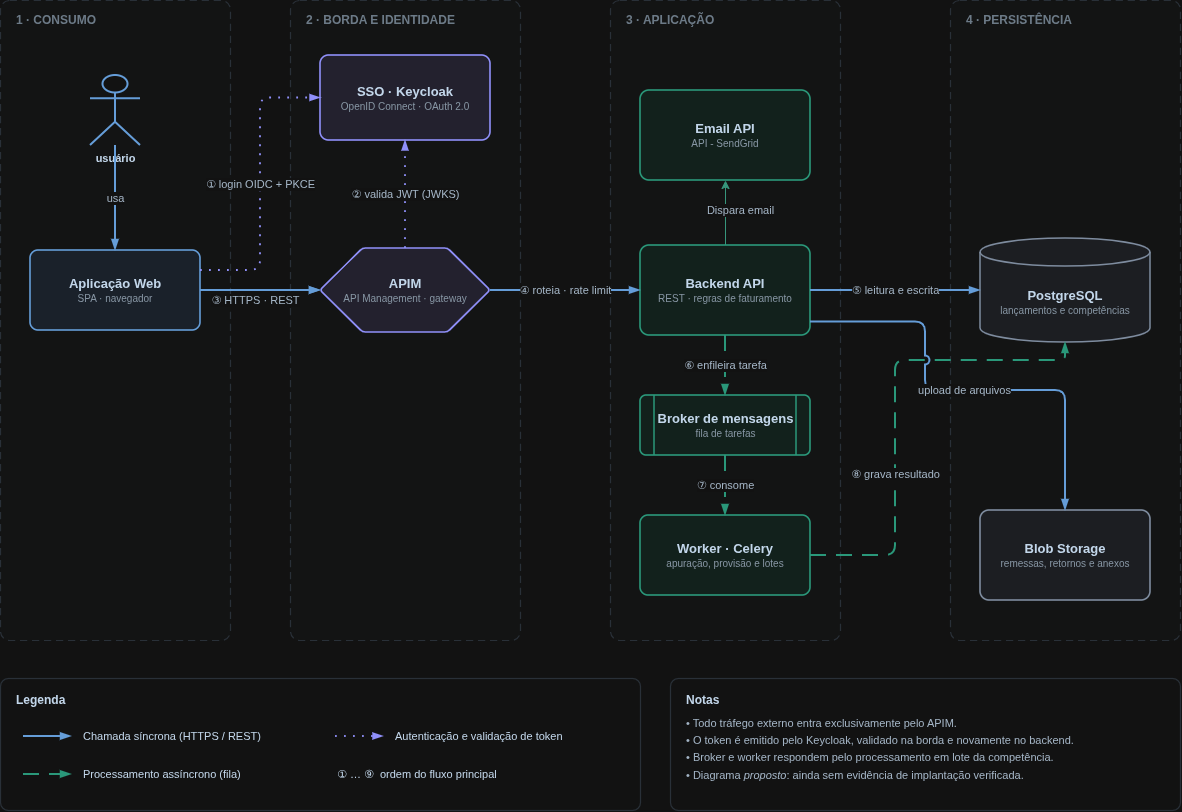
\includegraphics[width=0.85\textwidth]{figs/diagrama-fluxo-geral.png}
        \caption{Diagrama do fluxo geral}
        \label{fig:minha-imagem}
    \end{figure}
\end{frame}



\begin{frame}[plain]
    \centering

    \vspace{1.2cm}

    {\small \textbf{Obrigado!}}

\end{frame}
\end{document}
